% !TeX root = ../main.tex
% Add the above to each chapter to make compiling the PDF easier in some editors.

\chapter{Prototype implementation}\label{chapter:prototype implementation}

%Link to RQ4.
This chapter will introduce a prototypical implementation of a tool to cover the automated EAD process presented in chapter~\ref{chapter:approach}. To cover the requirements of the literature an existing open-source project \textbf{Pivio} was further developed to cover the presented requirements in subsection~\ref{subsection:derivationofrequirements}. \hl{Pivio}

\section{Motivation} 

Based on the findings during the literature research the implementation of a prototypical solution needs to covers  the technology trends that influence nowadays the EA documentation. Furthermore the prototypical solution requires an intergration of aspects such as agile development, cloud aspects and decomposition of legacy systems into application components or microservices. Concurrently with the literature review the existing open-source project Pivio was found that focuses on service discovery. This project was adapted and further developed to align it with the presented approach in section~\ref{chapter:approach}.

%Why Pivio?
\subsubsection{Pivio}
Pivio is a service registry. The main purpose of the project is to retrieve metadata of the deployed service. The information collected can be the name, owner and VCS information including runtime environment data and service dependencies.

Figure~\ref{fig:pivio-highlevel} shows the high level architecture of Pivio. The two main parts used in this approach of Pivio are:
\begin{itemize}
    \item Pivio web: A Webview
    \item Pivio server: A simple REST API connected to a schemaless database
\end{itemize}

The original open-source project was used as a solution for microservice discovery. During this work the project was extended to document an application during the application development pipeline and maintain this information.

\begin{figure}[htpb]
  \centering
  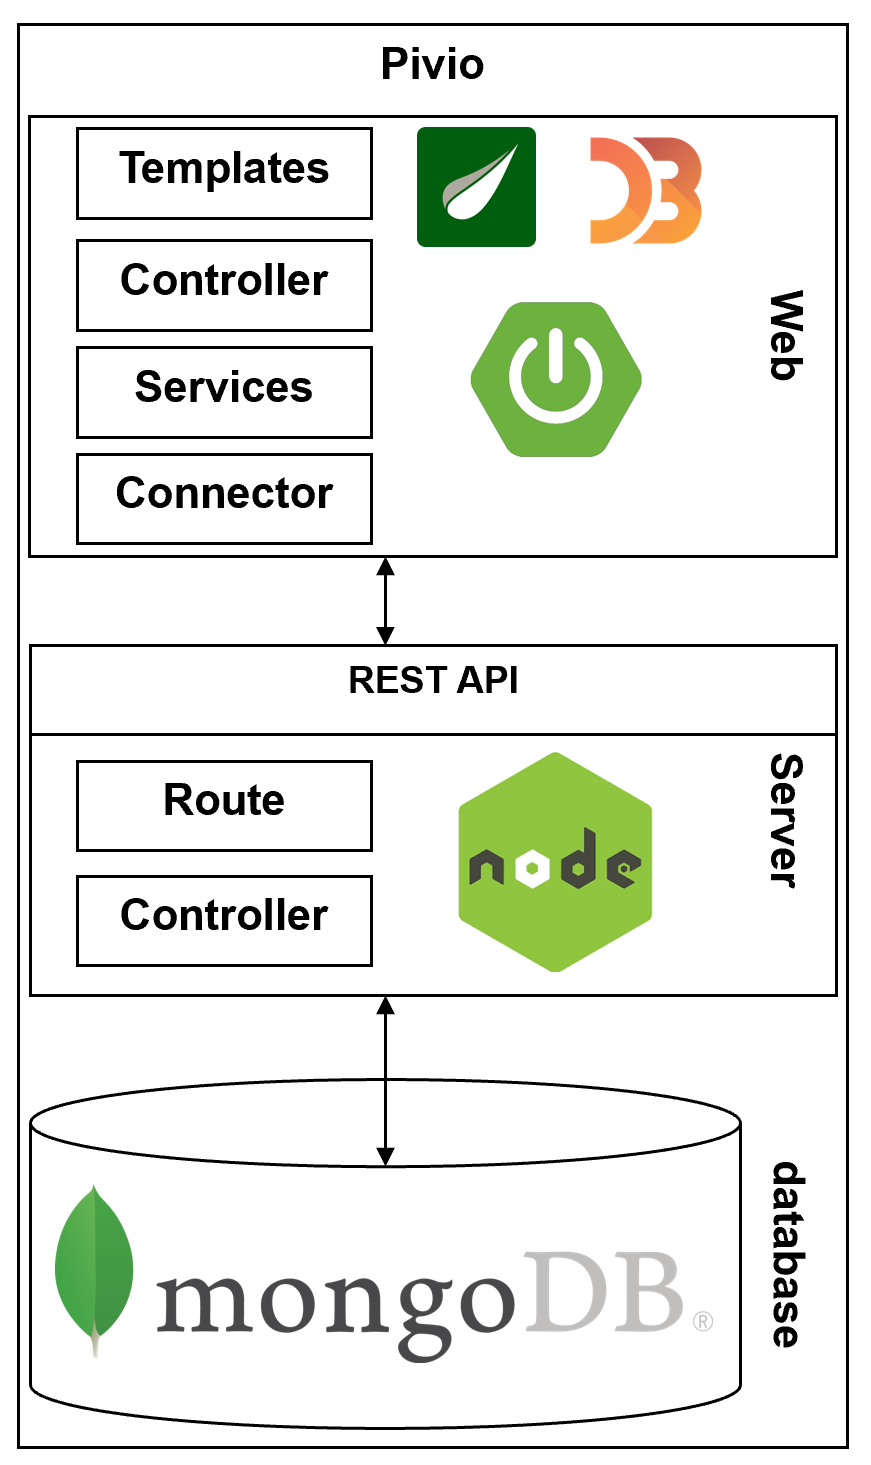
\includegraphics[width=0.5\textwidth]{figures/pivio-highlevel.PNG}
  \caption{High level architecture of Pivio}
  \label{fig:pivio-highlevel}
\end{figure}

%Technical requirements?

\section{Main views} 
This section will introduce the main views of the tool. The tool has three core views. The first view will be explained in subsection~\ref{subsection:overview}. It contains an overview of all artifacts that were documented according to the approach in chapter~\ref{chapter:approach}. The second view in subsection~\ref{subsection:detailedview} illustrates a detailed view of an artifact. The last view in subsection ~\ref{subsection:visualizations} shows different visualizations of the documented artifacts.

\subsection{Overview}\label{subsection:overview}

This subsection introduces the main page of the tool. The overview is divided into two parts. The first part displays a filter functionality described in ~\ref{subsubsection:filtertree}. The second part as shown in figure~\ref{fig:pivio-overview} shows the overview of the artifacts running on the cloud infrastructure.

Every artifact is displayed as a card. The cards contains the artifact name, the owner, the description of the artifact, the last changes of the artifact and the status. 
 
The status is depicted as a red or green circle. Red circles represents that the artifact has crashed or has been stopped. The green circle shows that the artifact is running. The status was added during this thesis. The goal of adding the status of the artifacts to the overview page is that the enterprise architects and other stakeholders can immediately react to a failure.

\subsubsection{Filter tree}\label{subsubsection:filtertree}

The filter tree was also implemented during this work. The main reason to add a filter functionality to the overview page was that more and more enterprises are moving their infrastructure to the cloud and therefore the amount of artifacts running on cloud environments has increased significantly.\hl{ Cloud Computing Survey. 2016}
An average enterprise has more than 900 artifacts hosted in a cloud infrastructure. \hl{Odun-Ayo} Therefore the implementation of a filter functionality in the overview page is seen as useful.

The filter contains the metadata of every artifact. The metadata includes several properties of the artifacts such as the name, the short name, the status, the description, the changes (last upload and last update), the domain, the subdomain, the product, the owner and the links to other tools. The filer functionality depicted as "Quick Search..." enables a search through all the metadata properties mentioned before.
A hierarchical tree was included as a visualization to enable an overview of artifacts per different areas. The hierarchical tree is structured in the following form: Cloud environment, domains, subdomains, products, artifacts belonging to the product and links to other tools. An example of the hierarchical view can be seen in figure~\ref{fig:pivio-overview-filtertree}. Clicking on a node expands or collapses the tree and updates the search box automatically with the metadata on the node and the list of artifacts gets updated as well.

\begin{figure}[htpb]
  \centering
  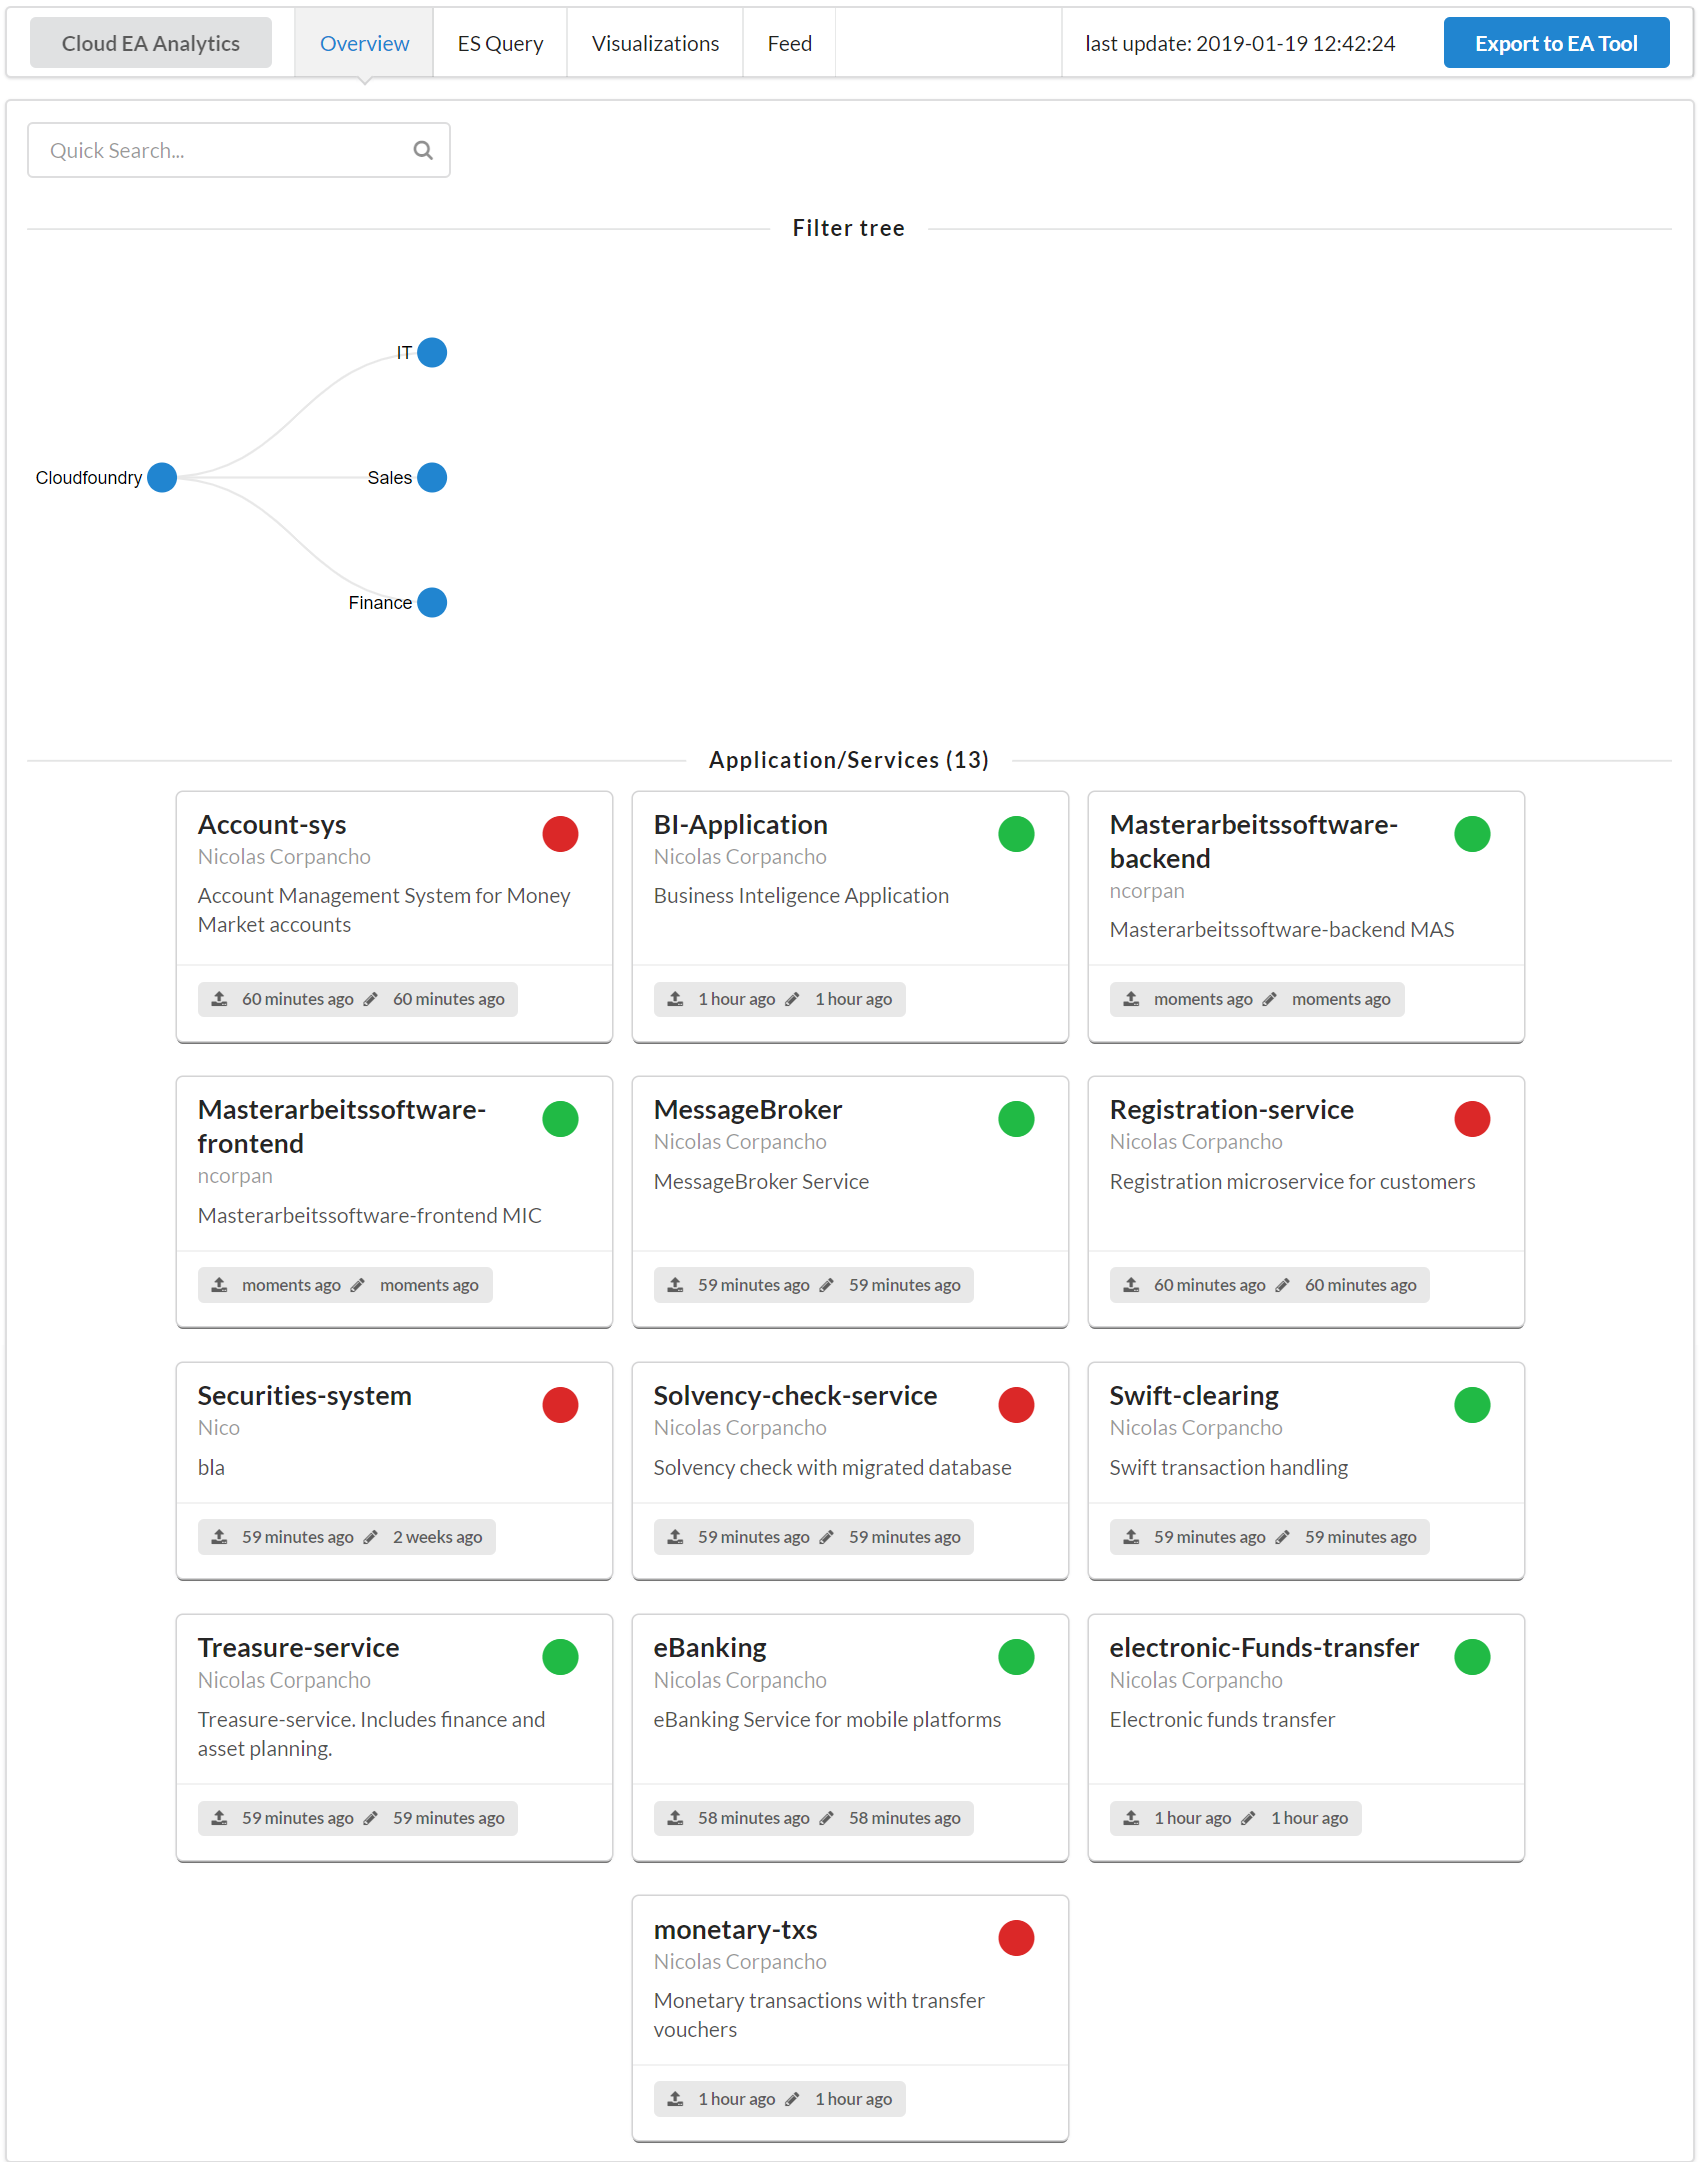
\includegraphics[width=1.0\textwidth]{figures/pivio-overview.png}
  \caption{Overview of the artifacts}
  \label{fig:pivio-overview}
\end{figure}

\begin{figure}[htpb]
  \centering
  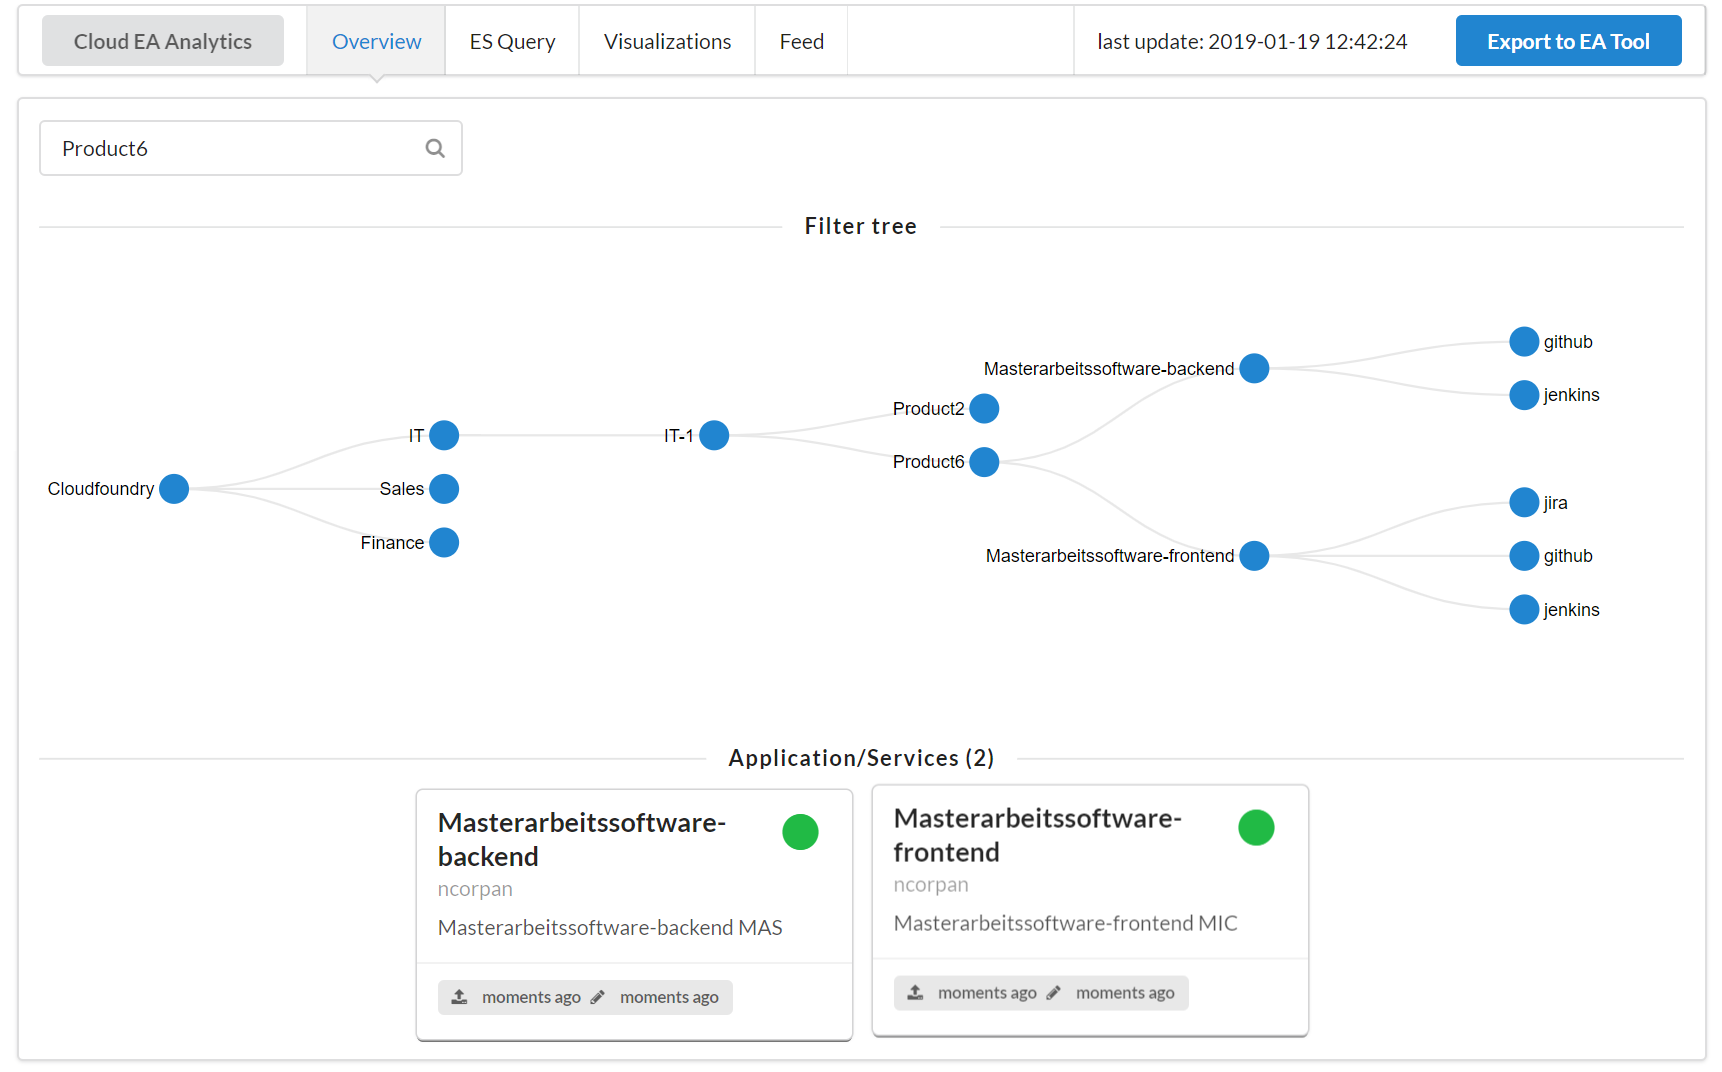
\includegraphics[width=0.8\textwidth]{figures/pivio-overview-filtertree.png}
  \caption{Filtertree in overview}
  \label{fig:pivio-overview-filtertree}
\end{figure}

\subsection{Detailed View}\label{subsection:detailedview}

The core view of the tool is the detailed view of an artifact. This view shows several properties and KPIs for one artifact. The main driver to cover a wide range of information regarding one artifact is to involve different stakeholder to use the tool.

The view is divided into nine sections. These sections are explained below.

%GENERAL SECTION SCREENSHOT
\begin{figure}[htpb]
  \centering
  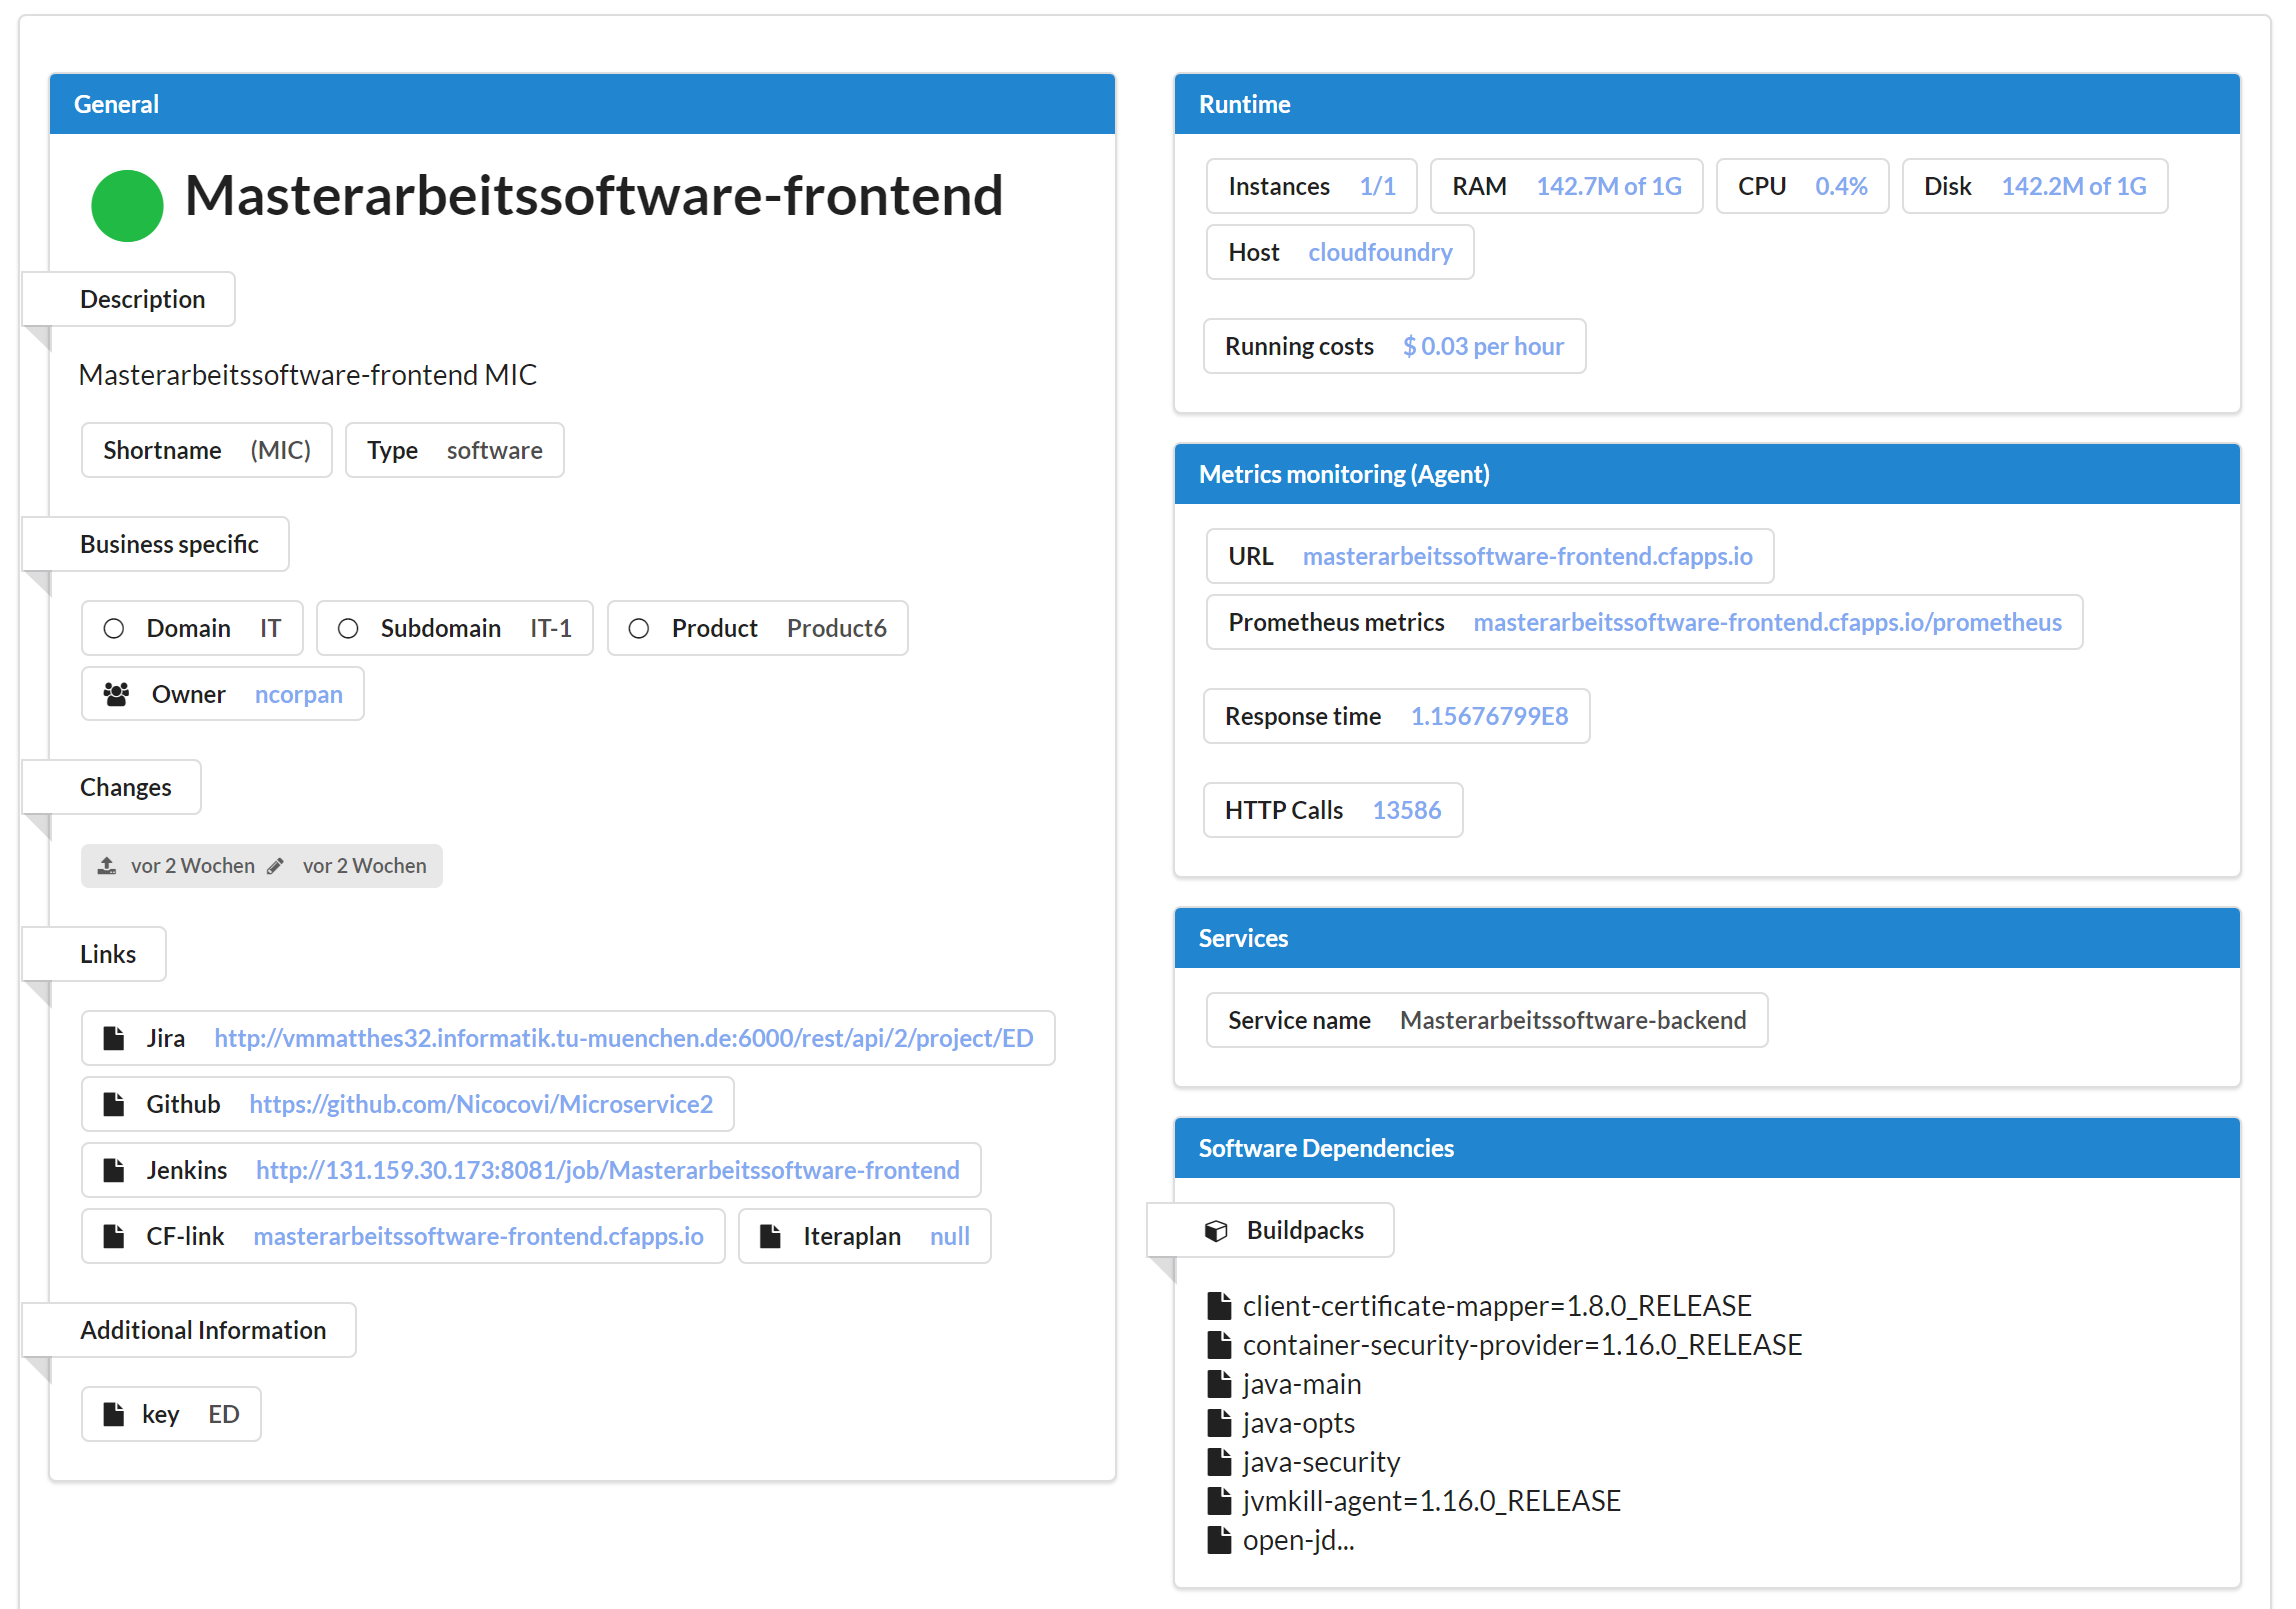
\includegraphics[width=1.0\textwidth]{figures/pivio-detailview-general.PNG} \caption{General section in Detailed View of artifact}
  \label{fig:pivio-detailedview-general}
\end{figure}

\subsubsection{General section}

This section shows general information about an artifact. Figure~\ref{fig:pivio-detailedview-general} shows this section. At the top of the section the status and the name of the artifact are shown. The description, the shortname and the type are retrieved from the PPM tool. 

The business specific information is gathered from the issues within the PPM tool. This information includes the business domains, subdomains and the product of the artifact. 

This section also contains the last changes of the documentation of the artifact and the date when the artifact was initially documented. The links to enable a federated enterprise architecture are also shown in this section. Further additional information is displayed too.

\subsubsection{Runtime section}

The runtime information is displayed on a separate section displayed in figure~\ref{fig:pivio-detailedview-general}. This information includes the number of instances of the artifact, the memory used, the CPU consumption and the disk required for the deployment of the artifact. It also includes the host type which means where the artifact is hosted since more than one cloud provider can be used.

In addition to the runtime behavior of the artifact, the running costs are calculated from the resource utilization. In this example the costs are calculated based on the memory per artifact instance. The cloud platform 
Cloudfoundry uses the unit "Gigabyte per hour" (GB-Hr) to calculate application costs. The rate used in this example is 0.03 dollar per GB-Hr. This means running an artifact that consumes 1 GB for 1 hour, the cost will be 0.03 dollar. The memory and duration are two parameters that can vary. This parameters determine the costs of the artifact. More instances increase the costs proportionally.

Additionally, cloud infrastructure resources can be allocated better based on the displayed resource consumption and the running costs of the application. The efficient allocation can lead to a decrease of infrastructure costs.

\subsubsection{Metrics monitoring section}

More use cases can be derived from monitoring and analyzing applications and their KPIs. \hl{Tilmann Rabl 2012} This is the reason why a section containing KPIs was added to the detailed view of an artifact. The metrics monitoring section is shown in figure ~\ref{fig:pivio-detailedview-general}.

The two selected KPIs for this section are the response-time and the number of http-calls of an artifact. The response-time KPI is displayed because it has different meanings. One of them is that a higher response time means an increased waiting time for the user. For that reason it is displayed to show a possible decreased performance of the system.
The total number of http-calls can be used for decommission purposes. If the artifact has high costs and total the number of call is low the enterprise architect should take measures.

This section also includes the link to the artifact and links to monitoring agents of the artifact. This agents are used to retrieve extra KPIs which are not covered by the monitoring tools offered by the cloud providers. 
%Nicht ganz einverstanden: offered through the API of cloud providers?
These agents show more technical KPIs such as heap memory consumption and java virtual machine information.
The links can be used by other stakeholder such as DevOps teams and CloudOps teams. This increases the involvement of stakeholders in regard to the tool.

\subsubsection{Services section}\label{subsubsection:servicessection}

The services section contains an overview of the services connected to the artifact shown in figure~\ref{fig:pivio-detailedview-general}. This section is used for dependency management of the artifact.

\subsubsection{Software dependencies section}\label{subsubsection:softwaredependenciessection}

The software dependency section illustrated in figure~\ref{fig:pivio-detailedview-general} is displayed to show the reliance of the artifact on other software packages. The presence of software dependencies are an important indicator of software complexity. 
A high degree of dependencies reflects the cohesion and coupling of the shown artifact, which can be seen as a software quality index. \hl{Wang}


%JIRA MONITORING SECTION SCREENSHOT
\begin{figure}[htpb]
  \centering
  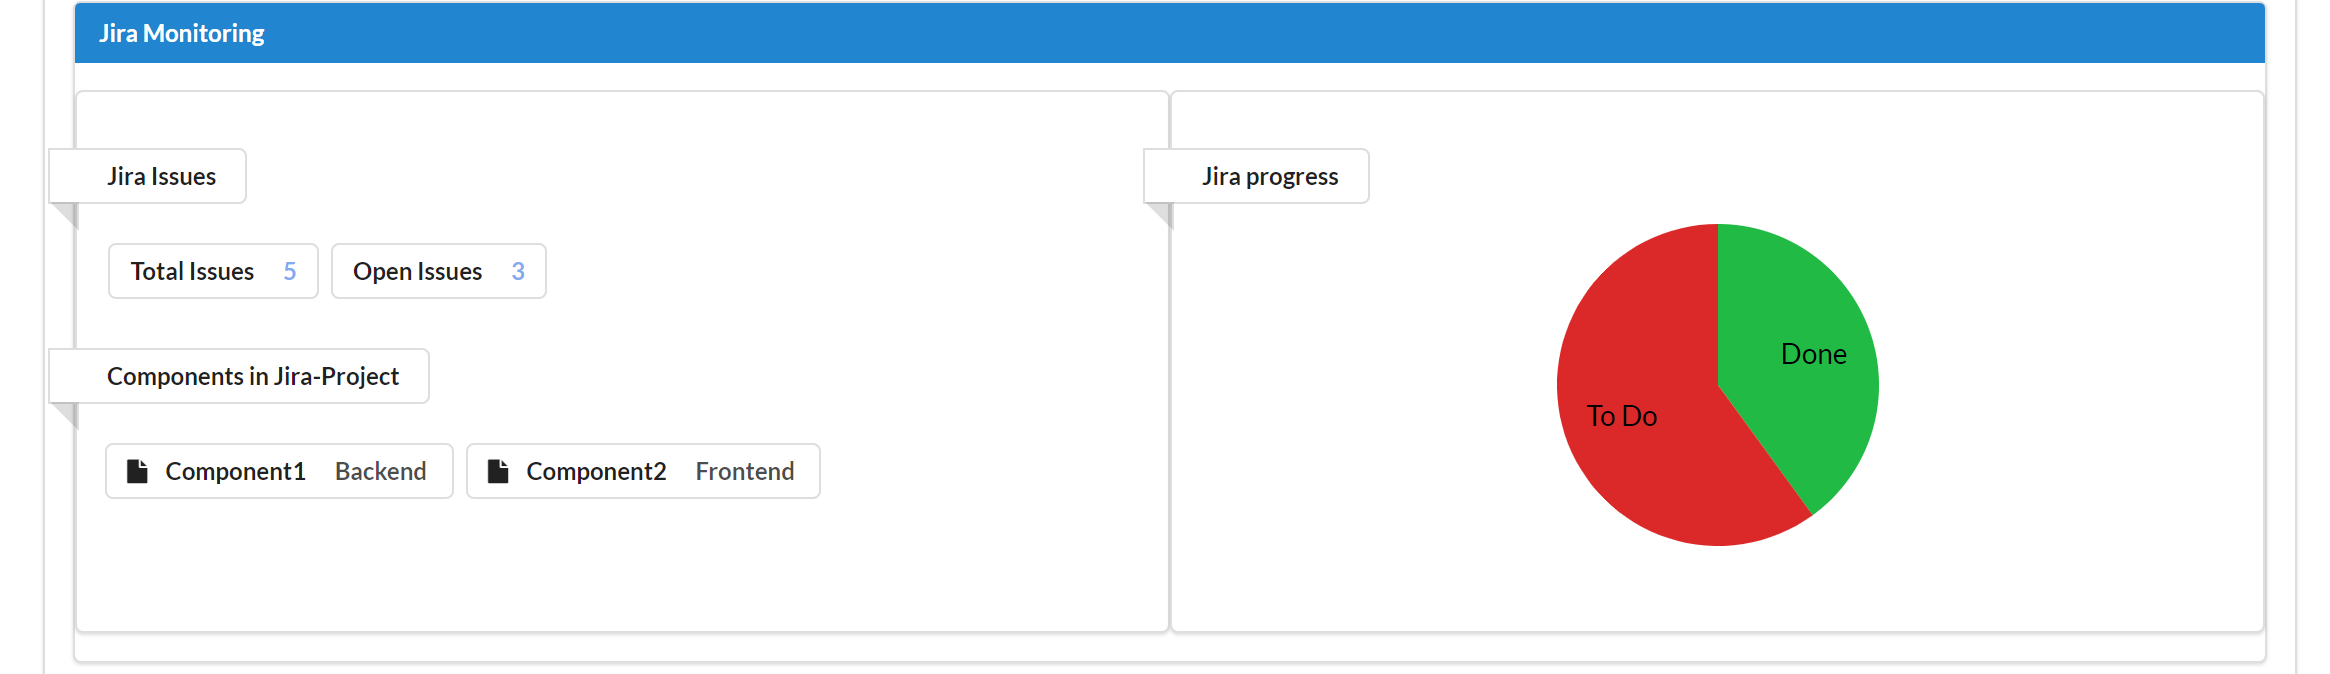
\includegraphics[width=1.0\textwidth]{figures/pivio-detailview-jira.PNG} \caption{Jira-Monitoring section in Detailed View of artifact}
  \label{fig:pivio-detailedview-jira}
\end{figure}

\subsubsection{Jira monitoring section}

This section displayed in figure~\ref{fig:pivio-detailedview-jira} shows the aggregated information of the PPM tool to the artifact. As mentioned in ~\ref{subsection:toolselection} Jira is used to manage projects. 

This section shows the development of the project in regard to the total amount of issues and the amount open issues. A pie chart was added in addition to visualize the progress. As named in ~\ref{subsubsection:getjirainformation} every Jira issue contains a standard field "component". The related components are displayed in this section to display other artifacts that are related to the parent application/product. The difference to the services section~\ref{subsubsection:servicessection} is that the shown artifact is not necessary connected to all services of the project. Other stakeholder like the product owner might have an interest to see all components/services of the project.

%GITHUB MONITORING SECTION SCREENSHOT
\begin{figure}[htpb]
  \centering
  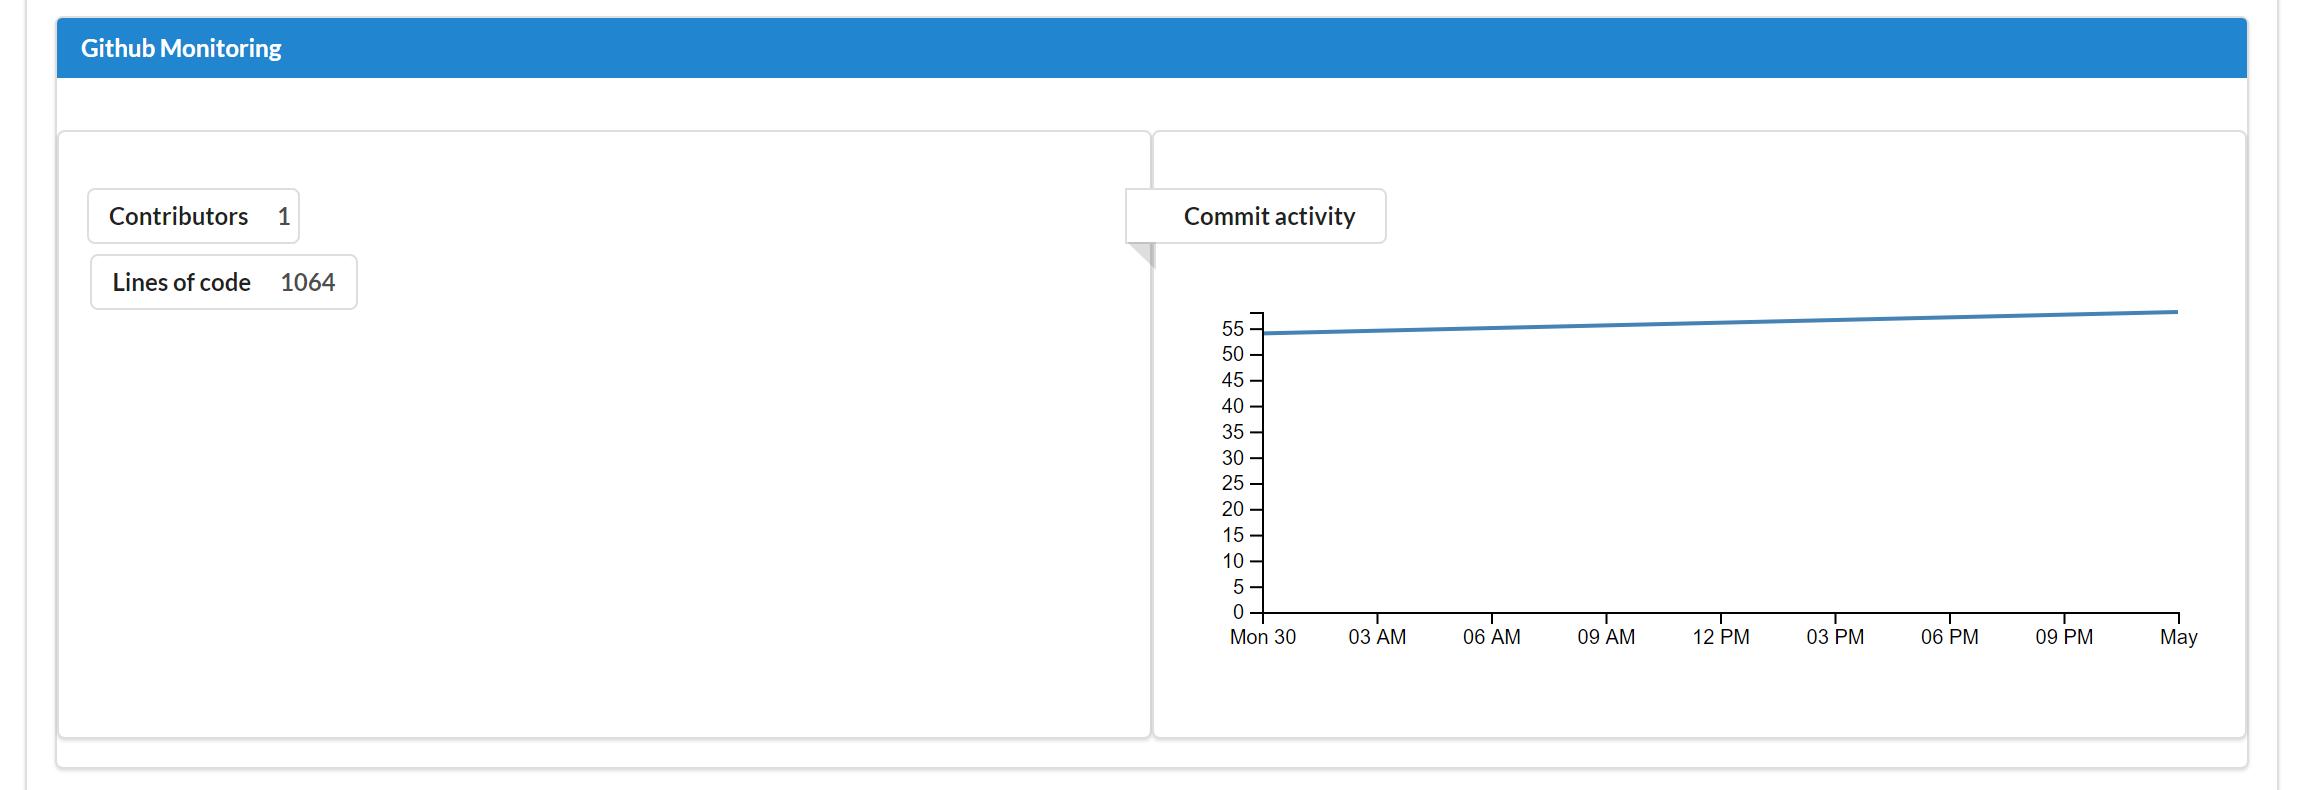
\includegraphics[width=1.0\textwidth]{figures/pivio-detailview-github.png} \caption{Github-Monitoring section in Detailed View of artifact}
  \label{fig:pivio-detailedview-github}
\end{figure}
\subsubsection{Github monitoring section}

Figure~\ref{fig:pivio-detailedview-github} shows the section of the VCS' repository. For demonstration purposes of the approach Github is used as the VCS.

This section is connected to the API of Github to show metrics of the repository. The metrics implemented during this work are the number of contributors of the repository and the lines of code. This KPIs serve as an indicator for the size of the service.

In combination with the Jira section the stakeholder can see the ongoing procedure and development of the project in one single page.

%JENKINS MONITORING SECTION SCREENSHOT
\begin{figure}[htpb]
  \centering
  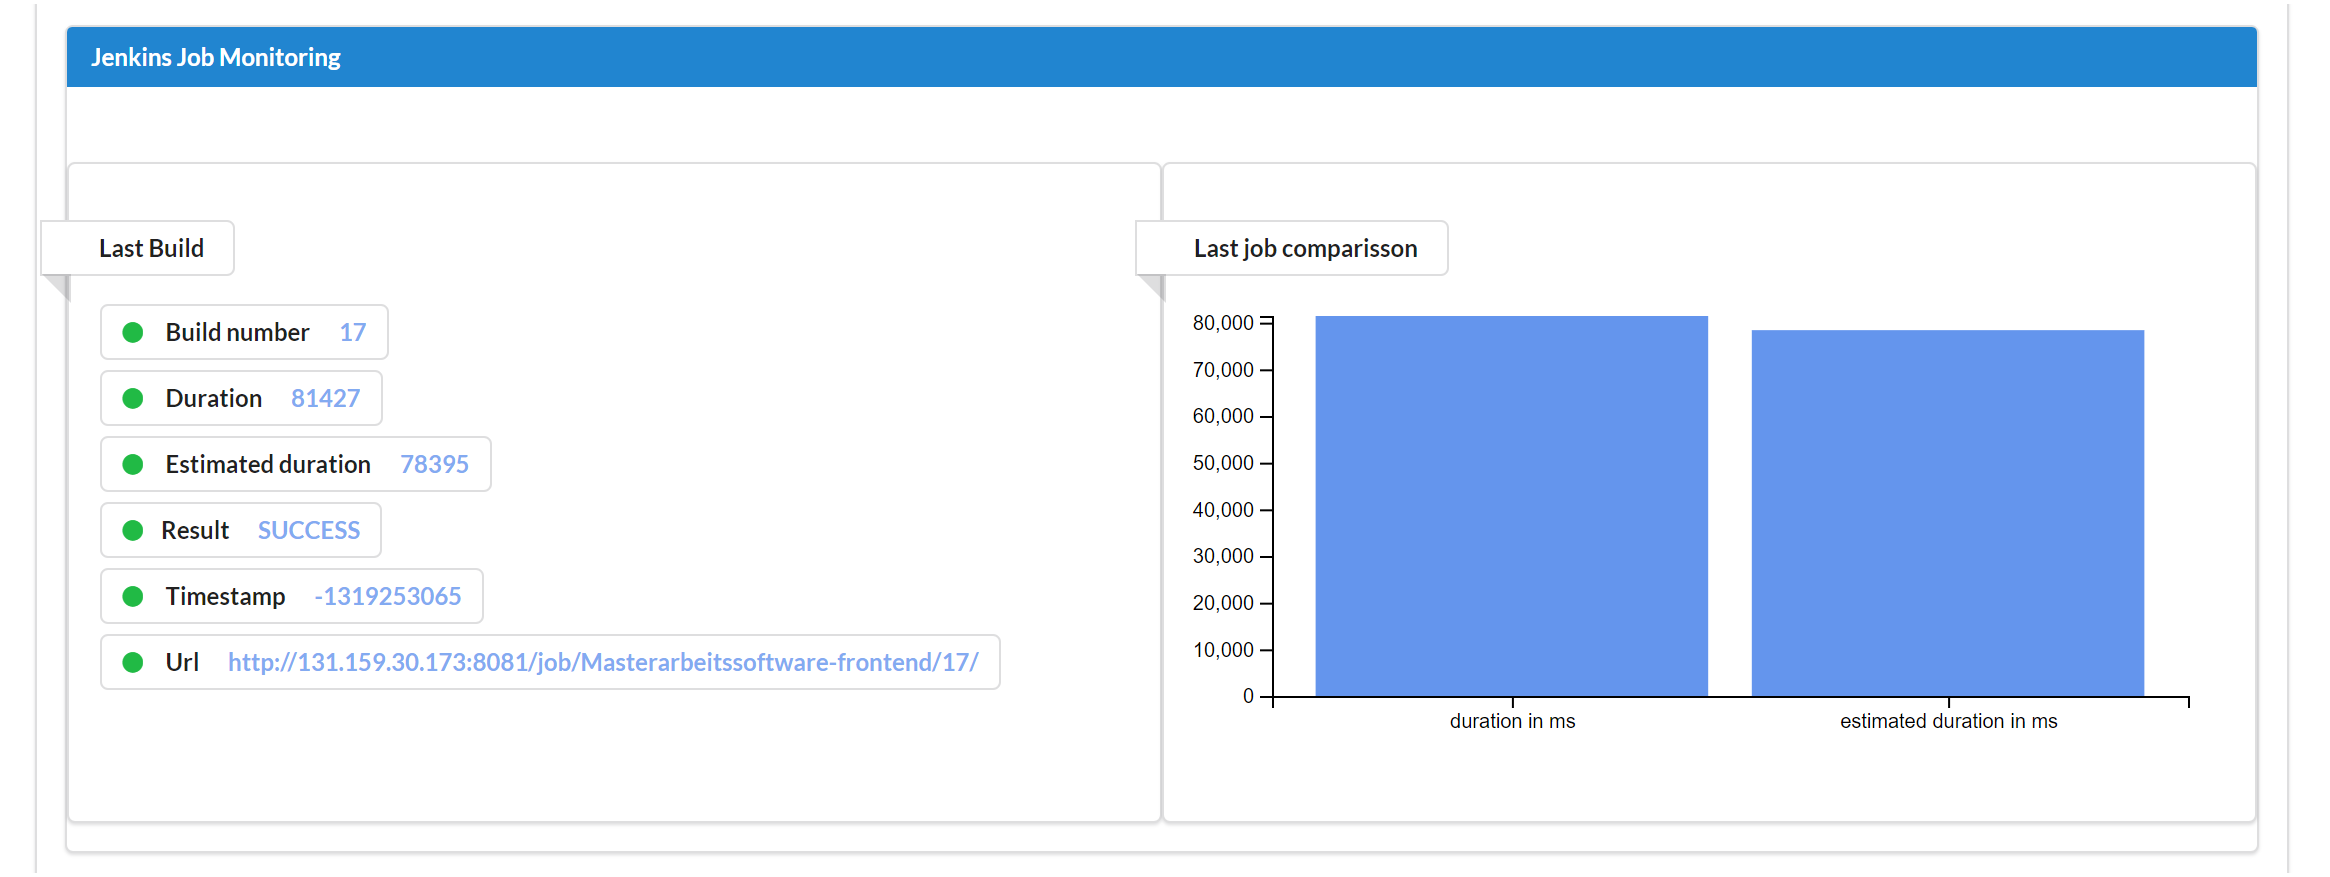
\includegraphics[width=1.0\textwidth]{figures/pivio-detailview-jenkins.png} \caption{Jenkins-Monitoring section in Detailed View of artifact}
  \label{fig:pivio-detailedview-jenkins}
\end{figure}
\subsubsection{Jenkins section}

Figure~\ref{fig:pivio-detailedview-jenkins} shows the section containing information of the CD/CI tool. Jenkins is used as the CI tool during this approach. The last build API of Jenkins is used to display information aboout the build deployment. This section contains on the left side the following metrics: the last build number, the duration of the last build, the estimated duration of the build process, the result of the last build, the timestamp and the url to the last build in the tool. On the right side it shows a bar chart comparing the duration of the last build and the estimated duration. The comparison is used to see whether the last build was affected by external factors such as latency or connection issues.

%ACTIONS SECTION SCREENSHOT
\begin{figure}[htpb]
  \centering
  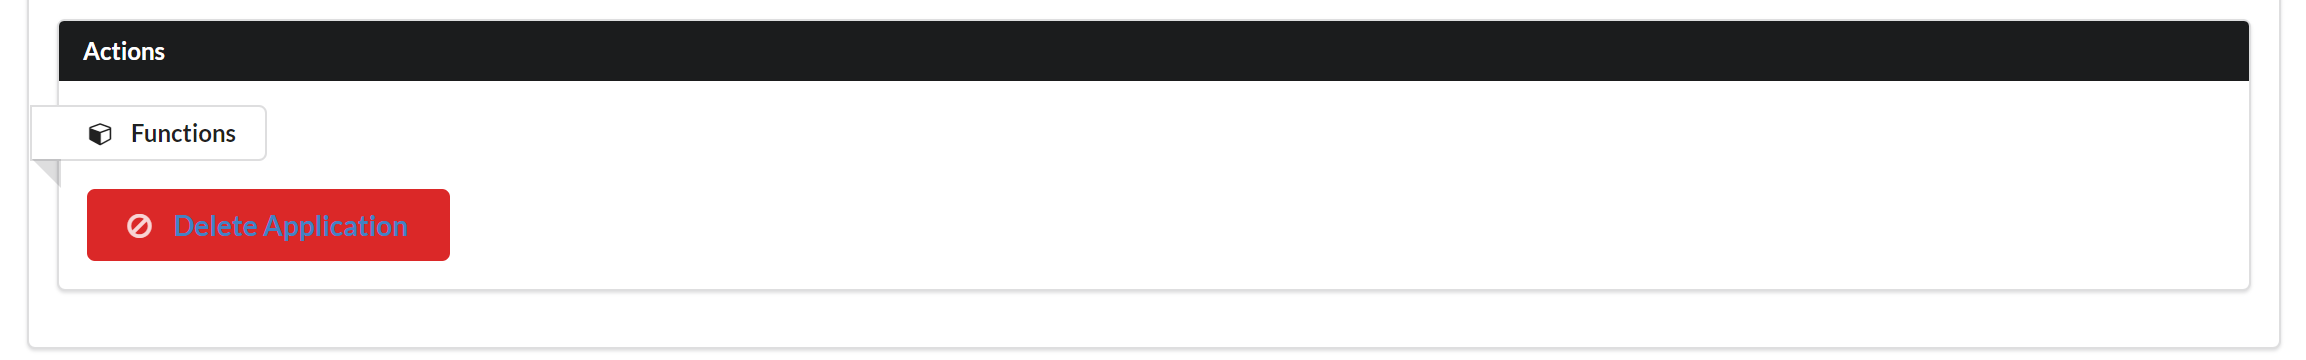
\includegraphics[width=1.0\textwidth]{figures/pivio-detailview-actions.PNG} \caption{Actions section in Detailed View of artifact}
  \label{fig:pivio-detailedview-actions}
\end{figure}
\subsubsection{Actions section}

The actions section displayed in figure~\ref{fig:pivio-detailedview-actions} includes the manual delete functionality of the artifact. Further functionality can be added in this section such as an update function for a manual information update to include additional data.

\subsection{Visualizations}\label{subsection:visualizations}

Another essential view of this tool is the visualizations view. The view was implemented during this thesis using the d3.js library for producing dynamic, interactive data visualizations in the web component.\hl{d3.js} The visualizations view is divided into two diagrams. The first diagram is a combination of a hierarchical edge bundling diagram and a sunburst diagram. The second visualizations is an adjacency matrix.

\subsubsection{Communications and business domain assignment diagram}

As already mentioned the "Communications and business domain assignment diagram" is a combination of hierarchical edge bundling diagram and a sunburst diagram. As shown in figure~\ref{fig:pivio-visualizations-communications} both diagrams have been used to achieve a unique visualization.

Every artifact listed in the tool is displayed around the business information. The blue lines represent the communication between the different services running on the cloud. The purpose of the diagram is to visualize the dependency between the services. By clicking on a service, the detail view of the service is displayed. Hovering a service highlights the connections (blue lines) and the dependent services of the hovered service.

In addition to the communications, a sunburst layout was developed to aggregate the business information. The domains and products of the displayed services are shown underneath the communications diagram allowing to visualize the assignment of the services to the products and the business domains. Due to this visualization it is easier to detect which other domains and products are affected if a service fails.

\begin{figure}[htpb]
  \centering
  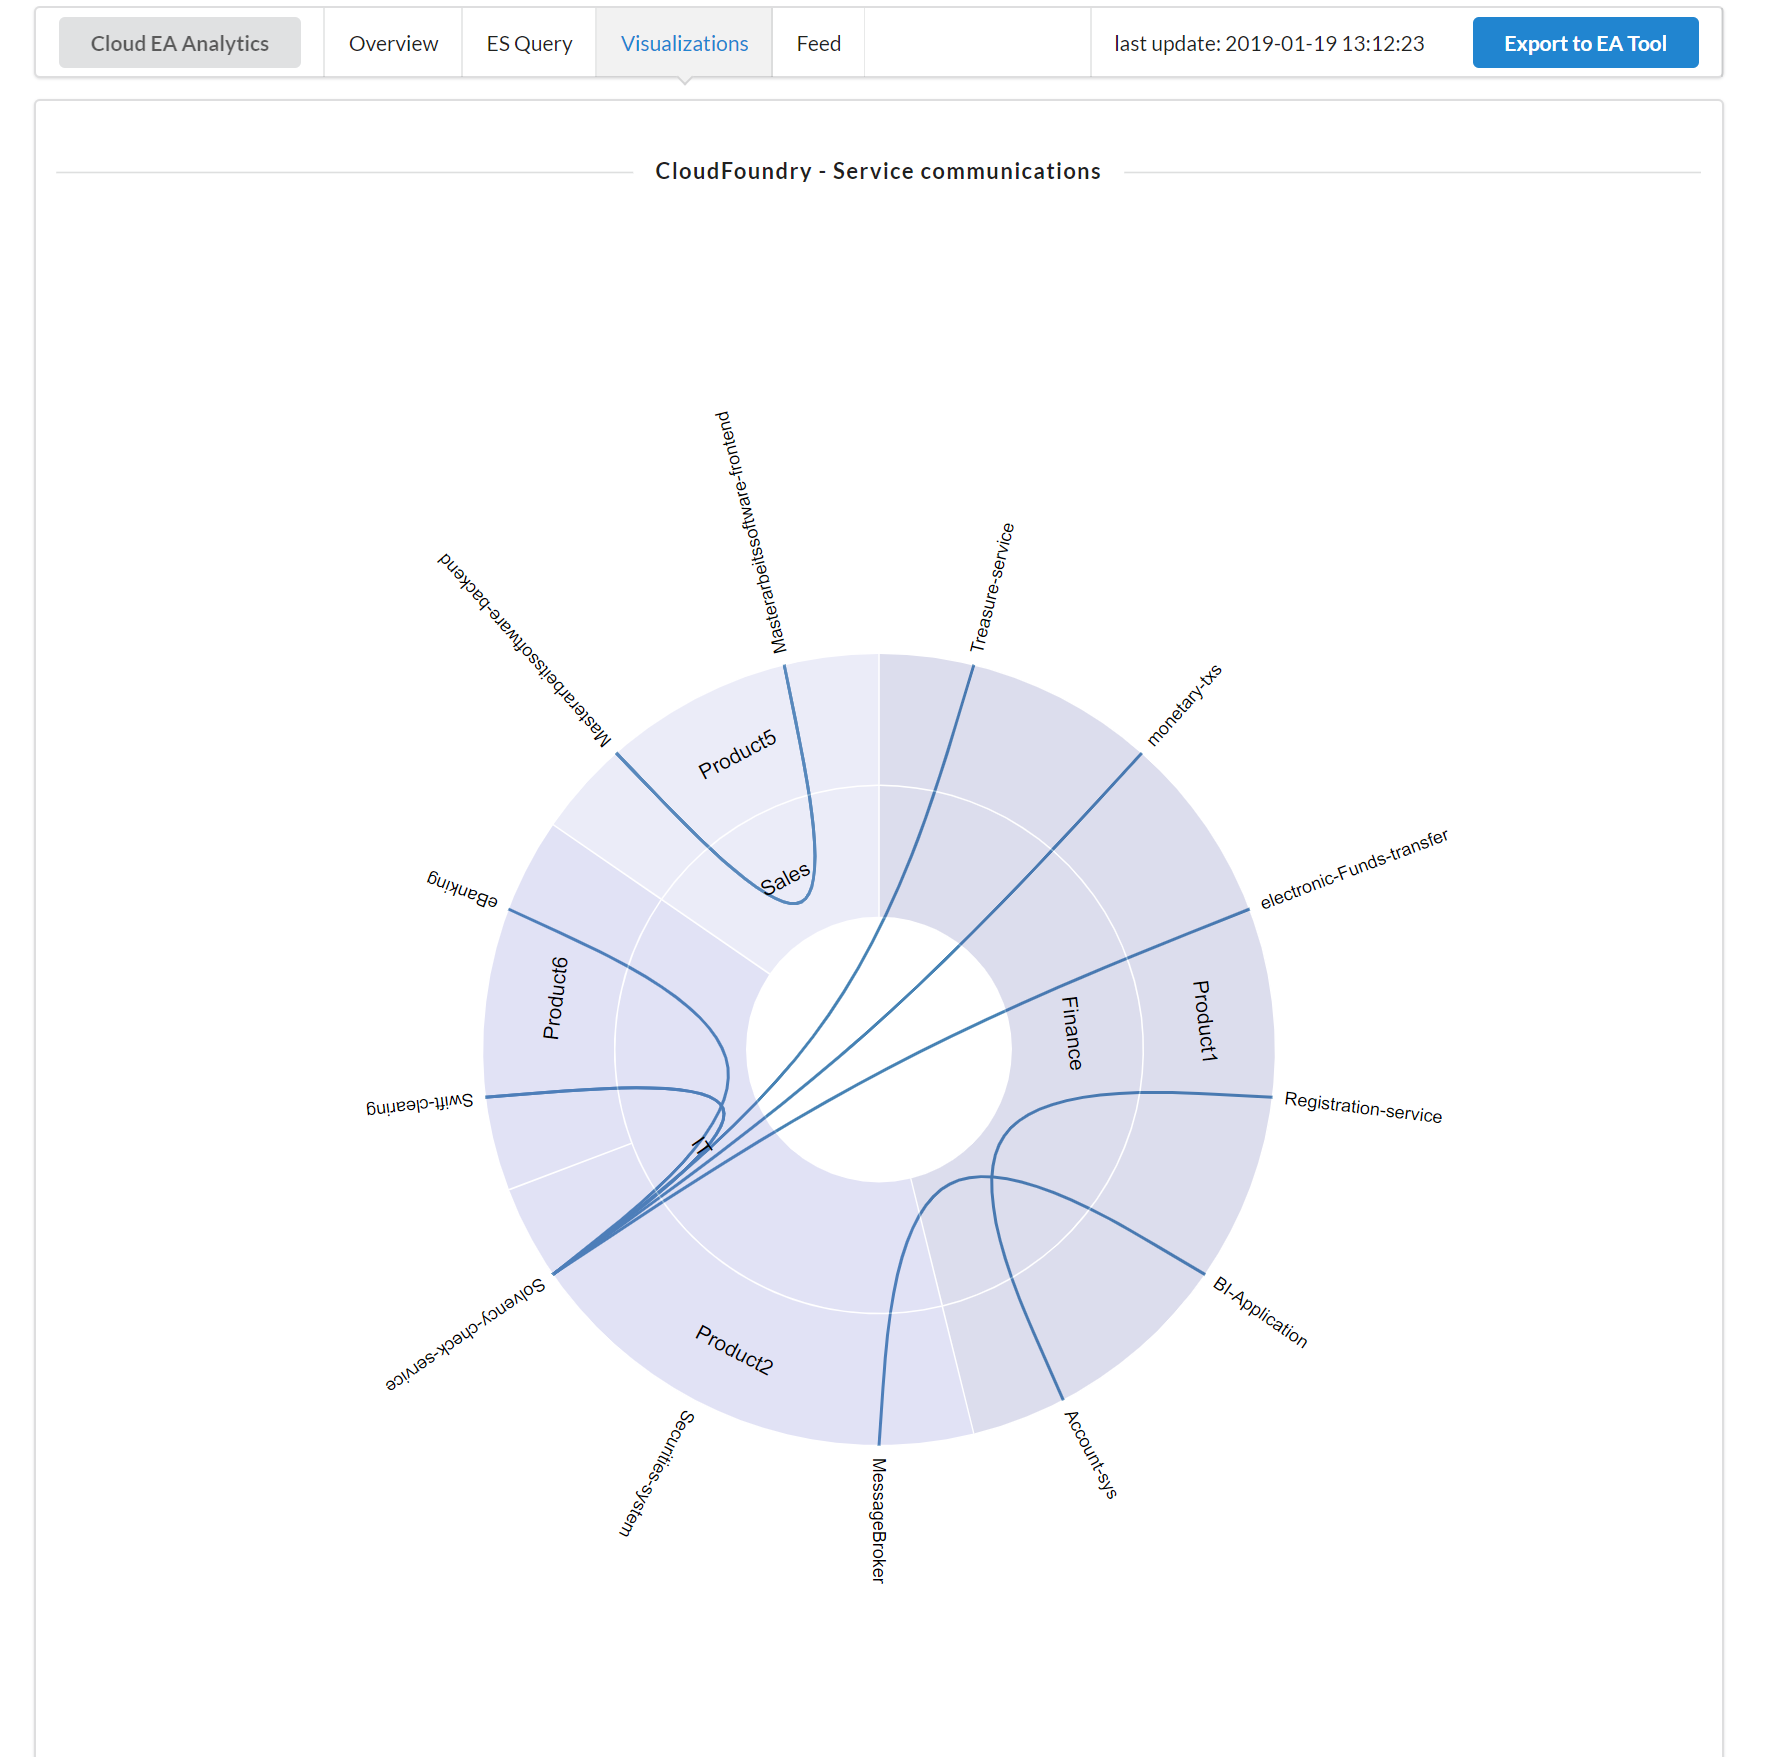
\includegraphics[width=1.0\textwidth]{figures/pivio-visualizations-communications.png}
  \caption{Communications and business domain assignment diagram}
  \label{fig:pivio-visualizations-communications}
\end{figure}

\subsubsection{Adjacency Matrix}

An adjacency matrix was developed to enable a dynamic diagram. The purpose of this matrix is to allow the possibility to rearrange the rows and columns regarding on different filter criteria. Figure~\ref{fig:pivio-visualizations-adjacency-matrix} shows the matrix ordered by the service with most dependencies (connections). The possible orders are:
\begin{itemize}
    \item by name
    \item by domain
    \item by frequency
\end{itemize}

Enabling the possibility to order by these criteria it is easier to visualize and analyze the dependencies of the services. The services with the most dependencies are always shown at the beginning of the matrix (left side).

By clicking on a cell it is possible to see the domains of the source service  and the destination service. This communication information box shown in figure~\ref{fig:pivio-visualizations-adjacency-matrix-cell} can be extended to include detailed information on the specific connection.

\begin{figure}[htpb]
  \centering
  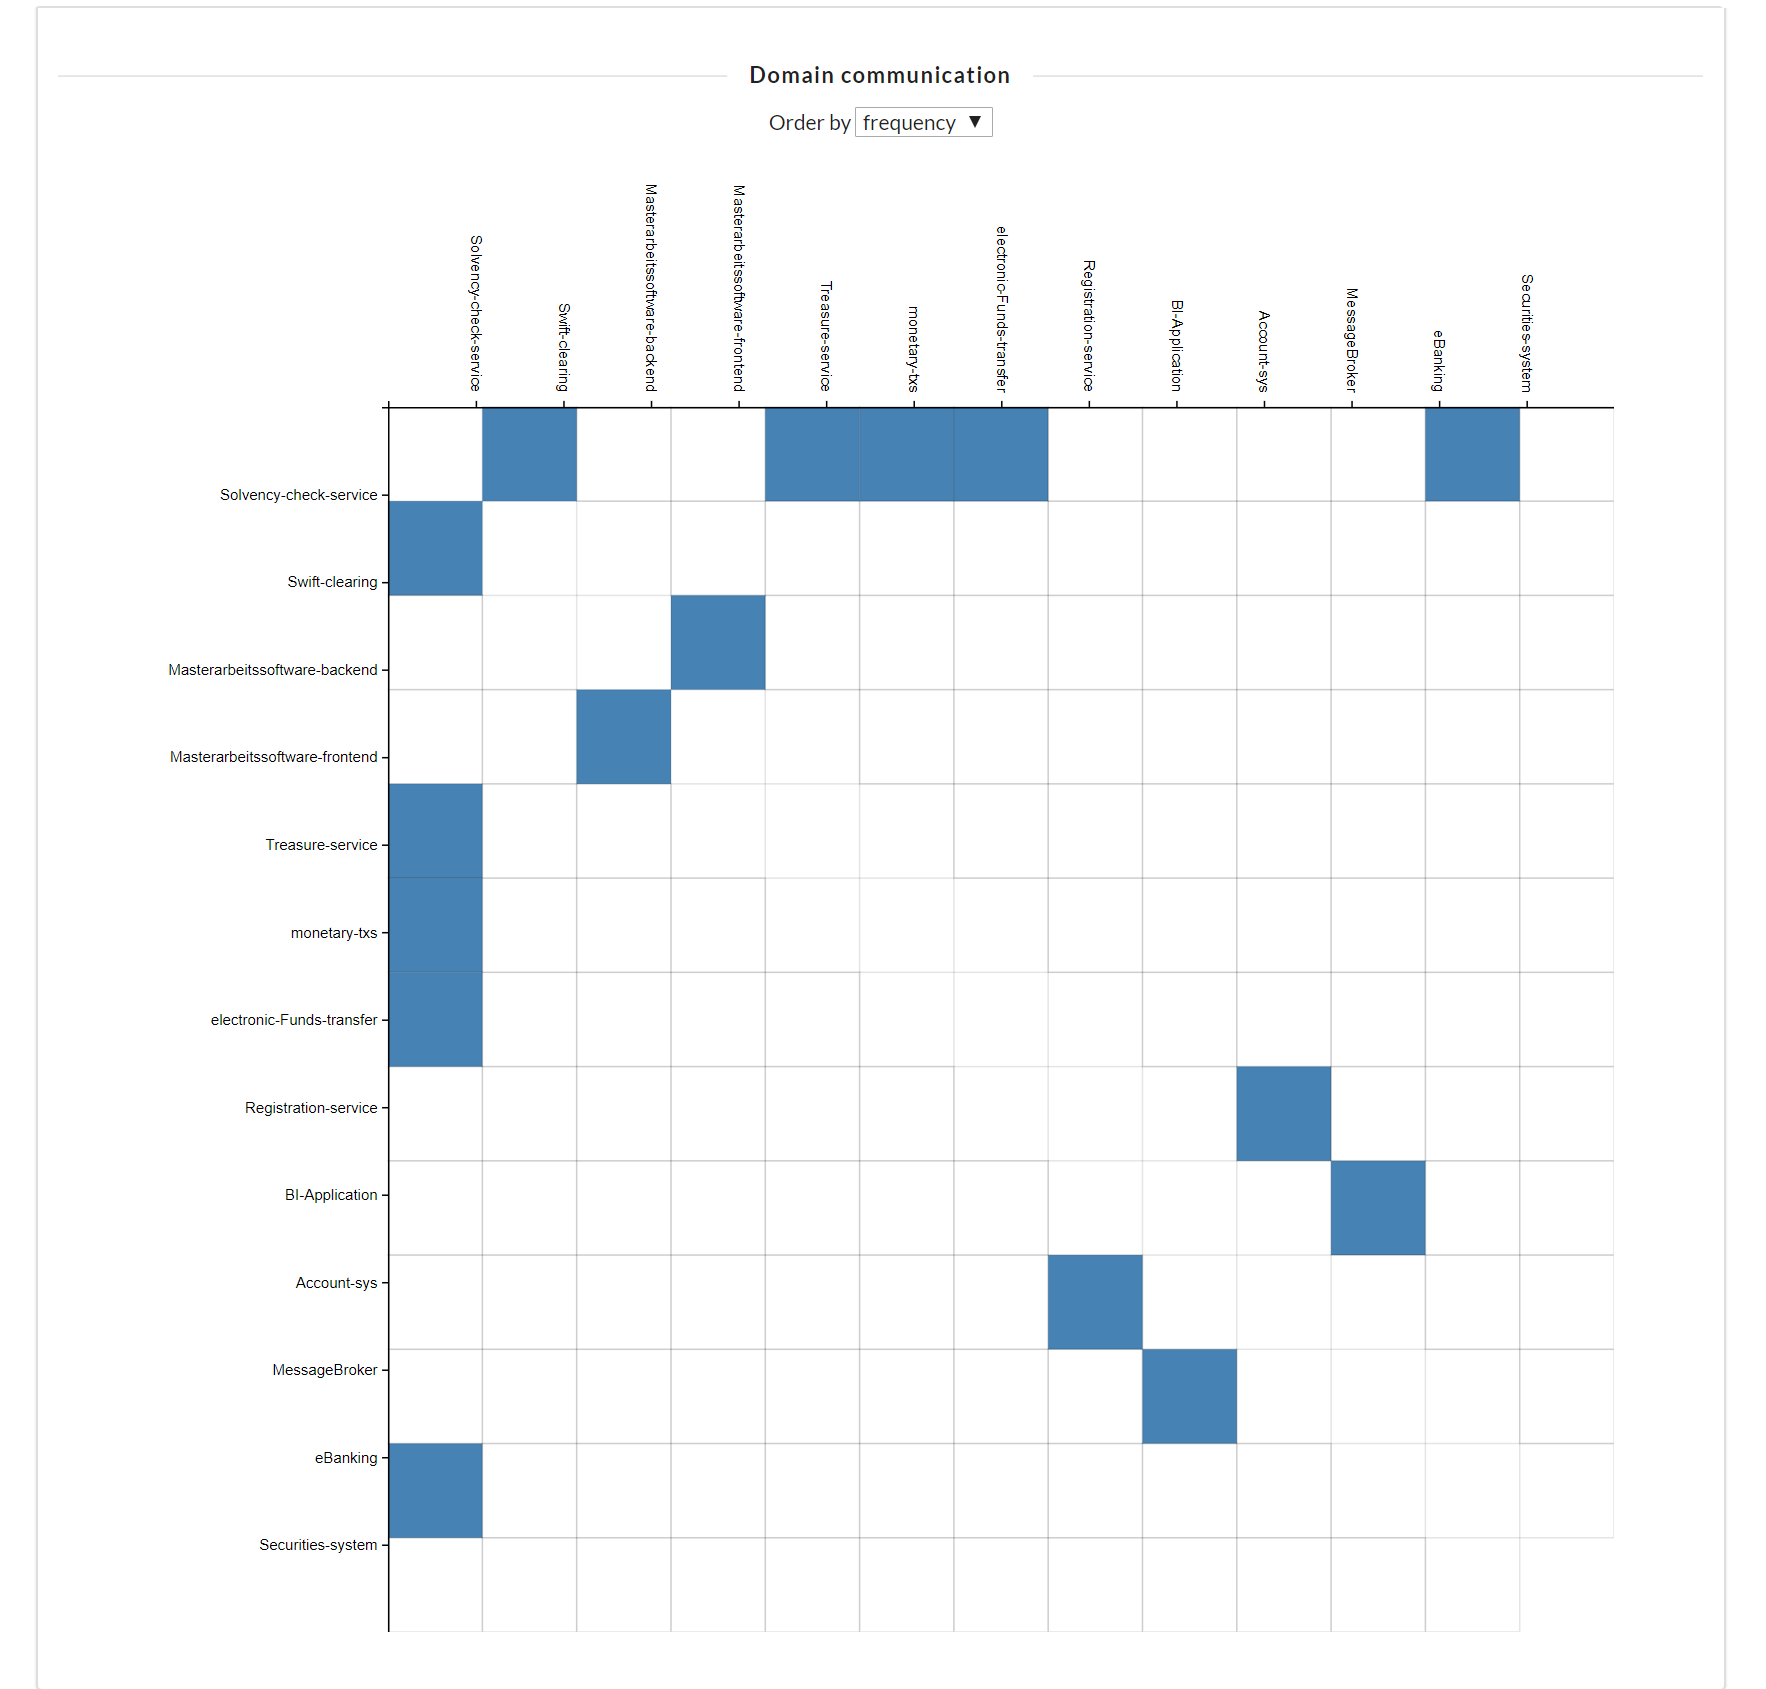
\includegraphics[width=1.0\textwidth]{figures/pivio-visualizations-matrix.png}
  \caption{Adjacency matrix}
  \label{fig:pivio-visualizations-adjacency-matrix}
\end{figure}

\begin{figure}[htpb]
  \centering
  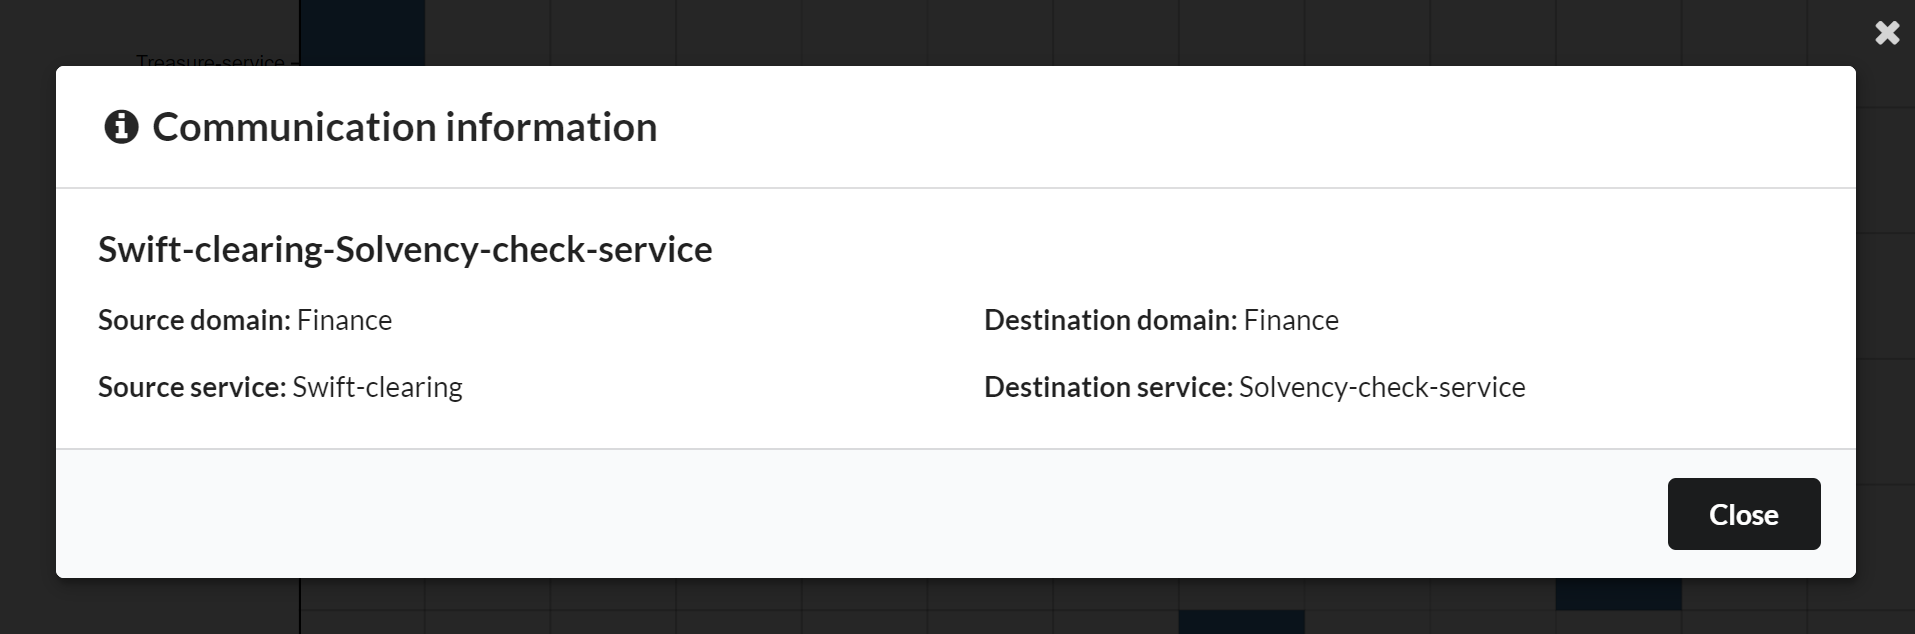
\includegraphics[width=1.0\textwidth]{figures/pivio-visualizations-matrix-cell.PNG}
  \caption{Adjacency matrix cell information box}
  \label{fig:pivio-visualizations-adjacency-matrix-cell}
\end{figure}

\section{Component diagrams}

This section shows two component diagrams of the two main components of the tool: Pivio web and Pivio server.

\subsection{Pivio web}

Figure~\ref{fig:pivioweb-component} shows the component UML diagram of the frontend component. The main component of Pivio web is the PivioServerConnector. This component contains the individual calls to the backend component. It uses the component ServerConfiguration to get the current server address. The ServerConfiguration is linked to the application properties file where the links are hold.

\begin{figure}[htpb]
  \centering
  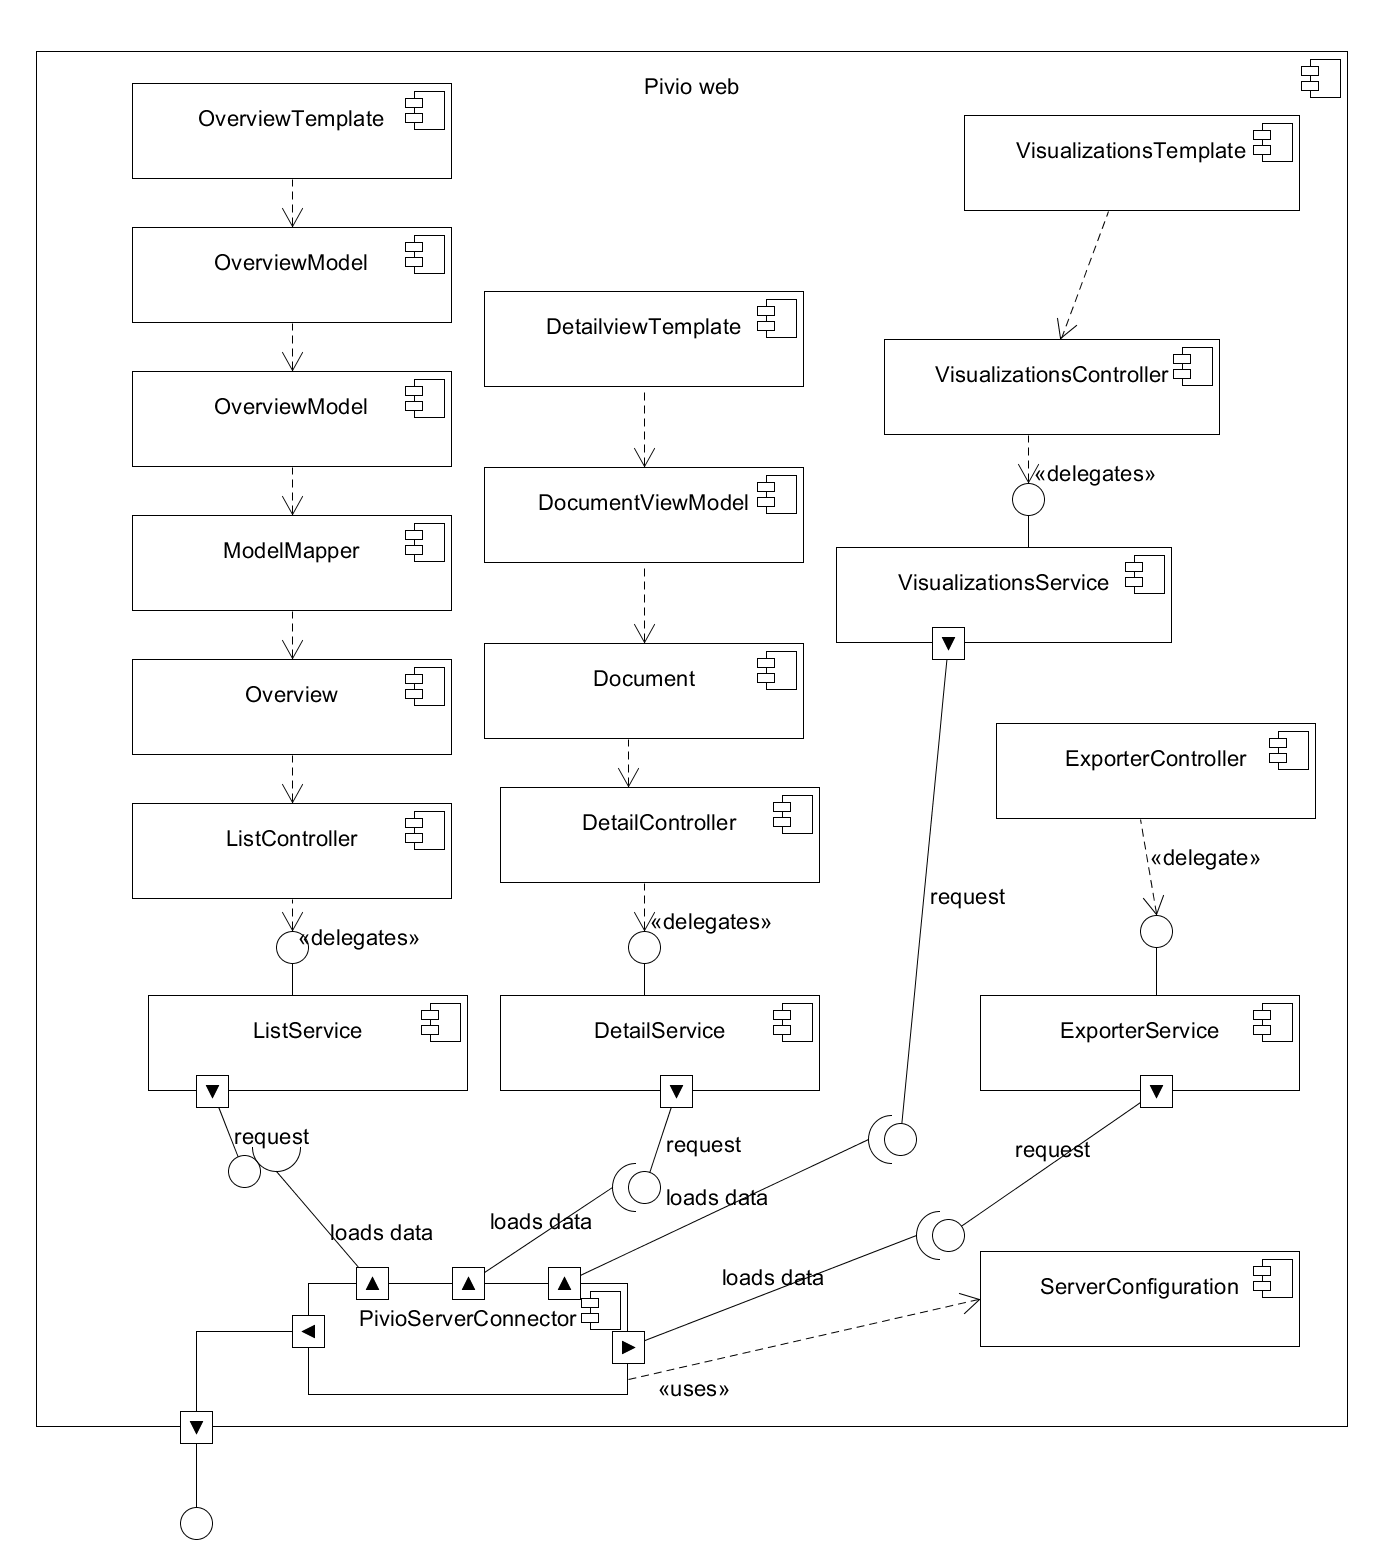
\includegraphics[width=1.0\textwidth]{figures/Pivioweb-ComponentDiagram.PNG}
  \caption{UML component diagram of Pivio web component}
  \label{fig:pivioweb-component}
\end{figure}

\subsection{Pivio server}

During this work the server component of Pivio was changed to a node.js application with a MongoDB database. Figure~\ref{fig:pivioserver-component} shows the UML component diagram.

The server component includes the main application component, and a controller, a route and a schema for storing applications into the database. The application component illustrated in figure~\ref{fig:pivioserver-component} as "App" defines the API paths and requires the "applicationRoutes" for forwarding the incoming calls. The "applicationRoutes" maps the implemented CRUD-Methods in the "applicationController" to the respective paths. The "applicationSchema" defines the model for the database and the controller requires it to validate and parse the incoming data. This data is stored in the MongoDB database component. 

\begin{figure}[htpb]
  \centering
  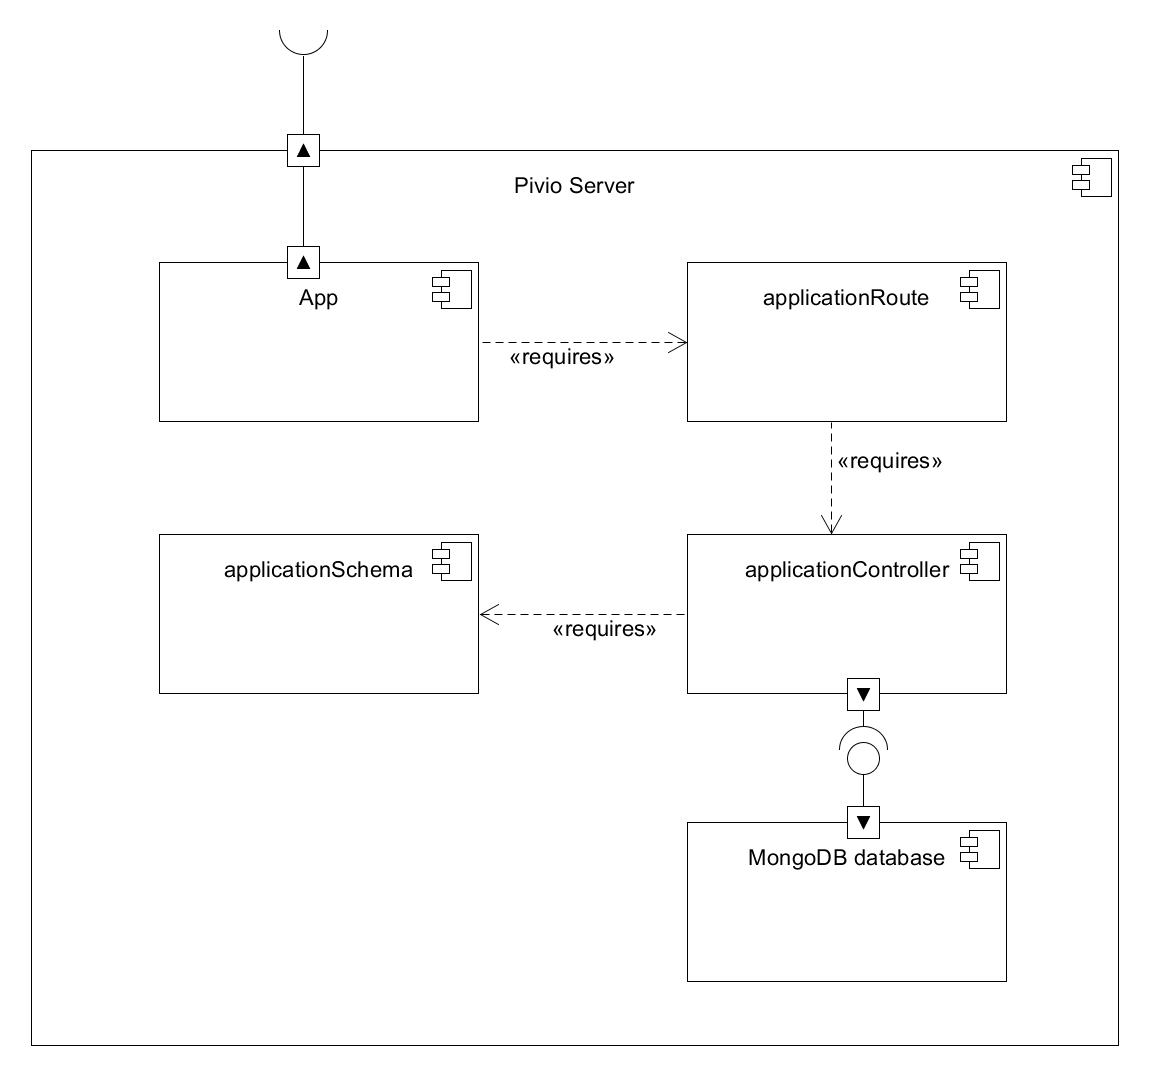
\includegraphics[width=1.0\textwidth]{figures/pivioserver-componentdiagram.PNG}
  \caption{UML component diagram of Pivio server component}
  \label{fig:pivioserver-component}
\end{figure}

\section{Class diagram}

The web component retrieves the data from the server component via a REST API. The return of the server is a JSON containing the properties of one service. This JSON response is mapped to the classes shown in figure~\ref{fig:server-response}.

Every response is mapped to a document. A document contains several properties. One of the properties is the information about the runtime. The runtime properties are modeled in a separate class. A document can contain one service which is composed by a list of buildpacks and one-to-many "Provides" objects. The list of buildpacks represents the list of software-dependencies mentioned in ~\ref{subsubsection:softwaredependenciessection}.
"Provides" objects are also modelled in a separate class. These objects represent the connection another service running on the cloud. The "Provides" class includes the service name, the protocol and the port of the communication.

The tools used during this approach are modeled as properties to facilitate the usage of the links. 

\begin{figure}[htpb]
  \centering
  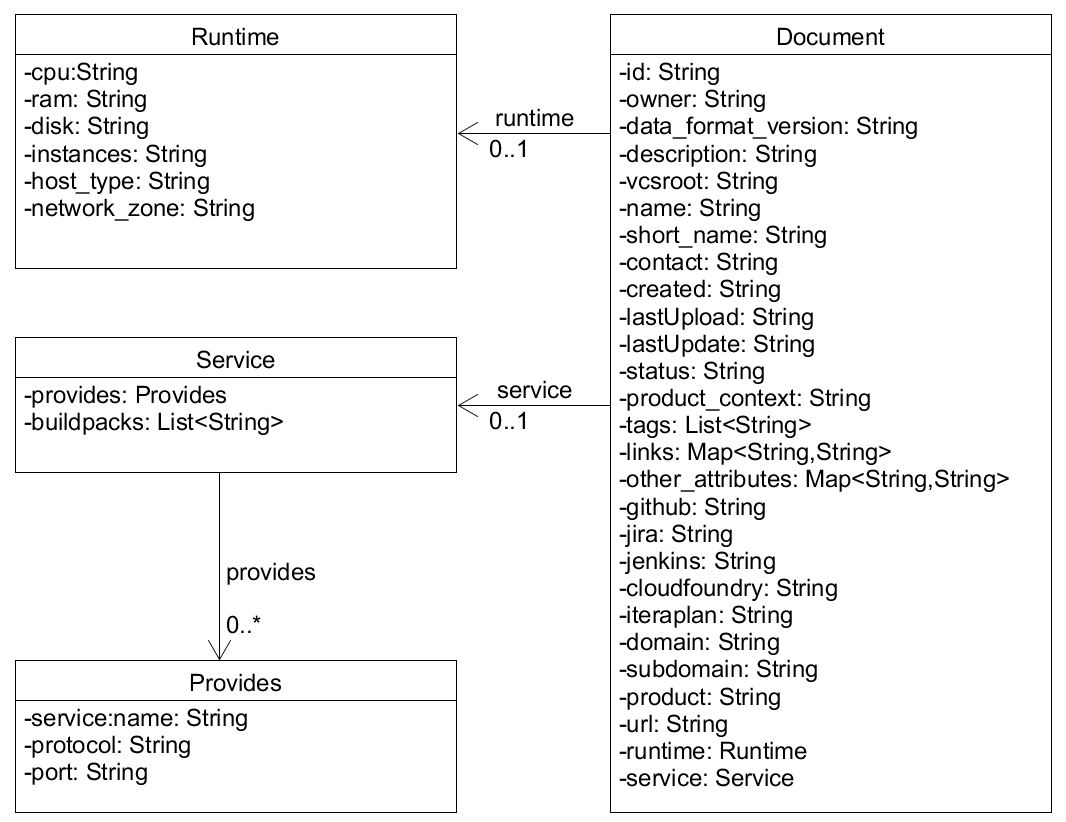
\includegraphics[width=1.0\textwidth]{figures/pivio-classdiagram.PNG}
  \caption{Class diagram of server response}
  \label{fig:server-response}
\end{figure}

% Jira Skript Ausnahmen
% anpassung in groovy. githublink
% httpSecurity.csrf().disable();












